\documentclass[aspectratio=169]{beamer}
\usetheme{Madrid}
\usepackage{booktabs}
\usepackage{graphicx}
\usepackage{array}

\title{Branch Specialization Checkpoint}
\subtitle{Conflict-Heavy Branch Routing}
\author{Branch Specialization Project}
\date{2026-05-22}

\begin{document}

\begin{frame}
  \titlepage
  \vspace{-0.5em}
  \begin{center}
    Checkpoint reason: direct role conflict still did not make unlabeled routing discover causal modularity.
  \end{center}
\end{frame}

\begin{frame}{Question}
  Prior result:
  \begin{itemize}
    \item entropy and load balancing did not reliably induce modularity;
    \item shrinking branches from 64 dims to 16 dims also did not help.
  \end{itemize}

  \vspace{0.8em}
  This checkpoint asks:

  \begin{quote}
    If the same query token requires incompatible predecessor-vs-successor
    lookups in different roles, does unlabeled routing pressure split the roles?
  \end{quote}
\end{frame}

\begin{frame}{Task Variant}
  Sample a prefix:
  \[
    [y_0, y_1, \ldots, y_{15}]
  \]

  \vspace{0.4em}
  The same query token is scored under two incompatible rules:

  \begin{center}
  \begin{tabular}{lll}
    \toprule
    Role & Query & Target \\
    \midrule
    Local & $y_i$ & $y_{i-1}$ \\
    Induction & $y_i$ & $y_{i+1}$ \\
    \bottomrule
  \end{tabular}
  \end{center}

  \vspace{0.4em}
  The task is designed so a single token-to-token lookup rule conflicts across roles.
\end{frame}

\begin{frame}{Metric Glossary}
  \begin{itemize}
    \item \textbf{Same top branch}: local and induction ablations hurt most when the same branch is removed.
    \item \textbf{Routed role match}: local's top causal branch is branch 0 and induction's top causal branch is branch 1.
    \item \textbf{Branch distance}: total-variation distance between local and induction causal branch distributions.
    \item \textbf{Gate routed match}: router probabilities point to branch 0 for local positions and branch 1 for induction positions.
  \end{itemize}
\end{frame}

\begin{frame}{Setup}
  Conflict-heavy local-vs-induction task:
  \begin{itemize}
    \item task variant: \texttt{bidirectional\_lookup};
    \item branch attention head dims: \texttt{[64]};
    \item equal local and induction loss weights;
    \item five seeds per condition, 1600 training steps;
    \item causal modularity measured by branch ablation.
  \end{itemize}

  \vspace{0.6em}
  Conditions: unconstrained learned token router, balance-only, entropy+balance,
  weak-label positive control, and oracle-route upper bound.
\end{frame}

\begin{frame}{Main Evidence}
  \begin{center}
  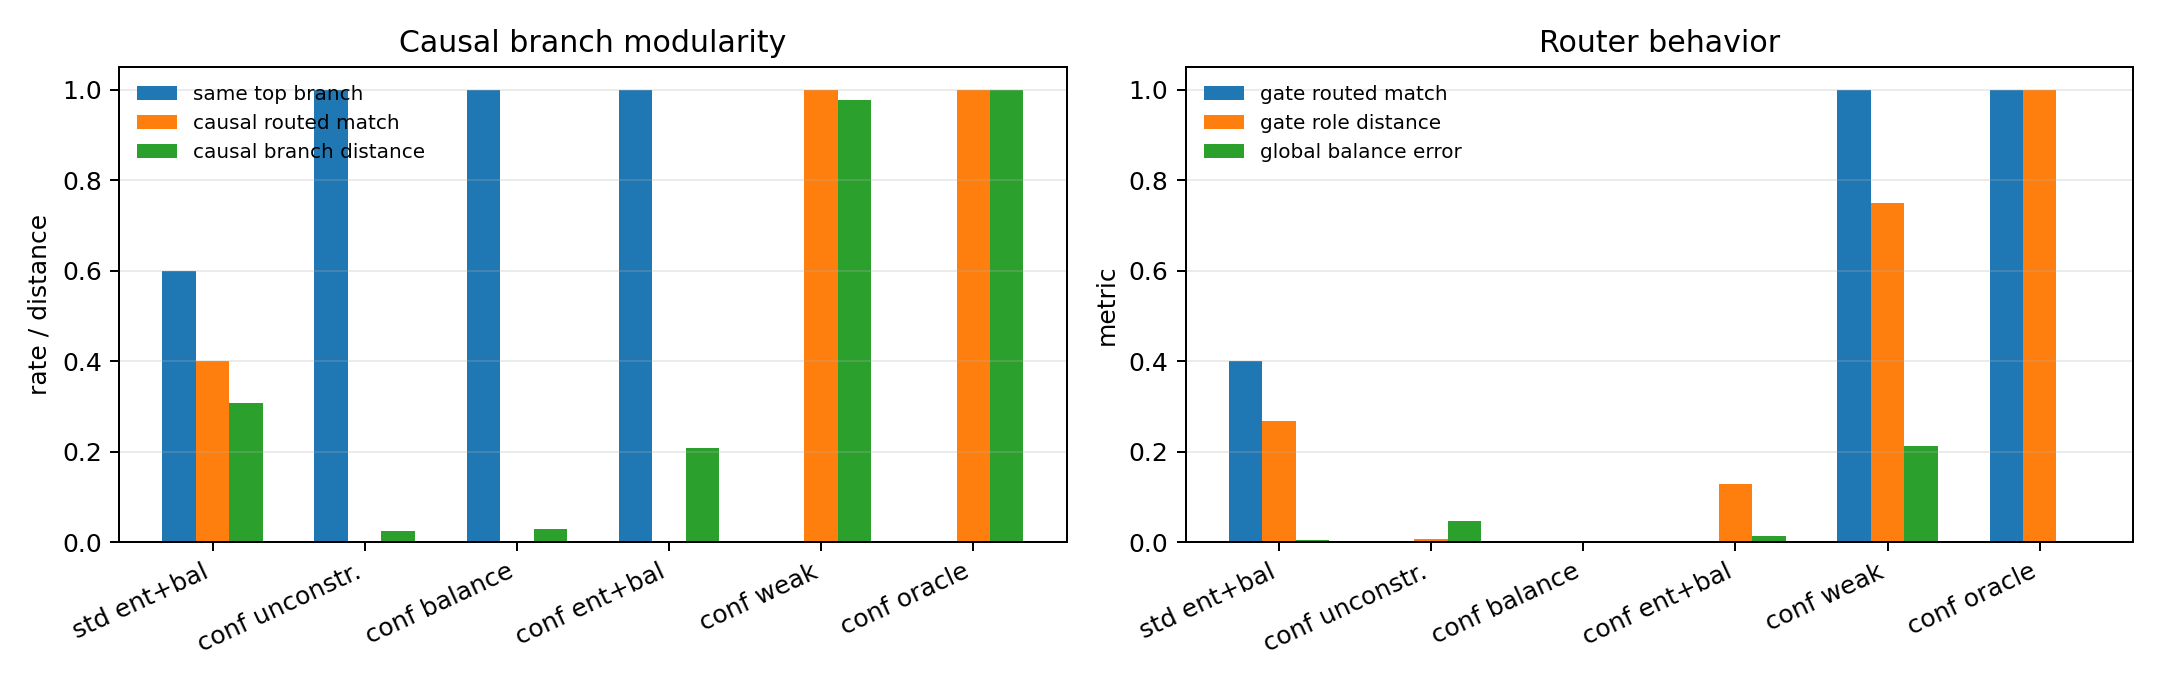
\includegraphics[width=0.92\linewidth]{figures/conflict_router_comparison.png}
  \end{center}

  \vspace{-0.4em}
  \small
  Conflict does not rescue unlabeled modularity. Weak labels and oracle routing
  produce clean causal role splits.
\end{frame}

\begin{frame}{Conflict Results}
  \begin{center}
  \scriptsize
  \begin{tabular}{lrrrrr}
    \toprule
    Condition & Local acc. & Ind. acc. & Same top & Routed match & Branch dist. \\
    \midrule
    \texttt{unconstrained} & 0.9992 & 1.0000 & 1.00 & 0.00 & 0.0237 \\
    \texttt{balance only} & 0.9991 & 0.9994 & 1.00 & 0.00 & 0.0283 \\
    \texttt{entropy+balance} & 0.9997 & 0.9998 & 1.00 & 0.00 & 0.2069 \\
    \texttt{weak label} & 0.9986 & 0.9997 & 0.00 & 1.00 & 0.9773 \\
    \texttt{oracle route} & 0.9994 & 0.9995 & 0.00 & 1.00 & 1.0000 \\
    \bottomrule
  \end{tabular}
  \end{center}

  \vspace{0.5em}
  All conditions solve the task, so the unlabeled failure is not a learnability failure.
\end{frame}

\begin{frame}{Comparison to Standard Task}
  \begin{center}
  \scriptsize
  \begin{tabular}{lrr}
    \toprule
    Condition & Routed match & Branch dist. \\
    \midrule
    standard wide64 entropy+balance & 0.40 & 0.3082 \\
    conflict wide64 entropy+balance & 0.00 & 0.2069 \\
    standard wide64 weak label & 1.00 & 0.8957 \\
    conflict wide64 weak label & 1.00 & 0.9773 \\
    conflict wide64 oracle route & 1.00 & 1.0000 \\
    \bottomrule
  \end{tabular}
  \end{center}

  \vspace{0.7em}
  Direct role conflict made the task stricter, but did not create spontaneous
  unlabeled causal modularity.
\end{frame}

\begin{frame}{Interpretation}
  \textbf{Supported:}
  \begin{itemize}
    \item Conflict task is learnable.
    \item Correct routing is sufficient for clean modularity.
    \item Weak role-informative routing pressure is sufficient.
  \end{itemize}

  \vspace{0.6em}
  \textbf{Not supported:}
  \begin{itemize}
    \item direct predecessor-vs-successor conflict plus generic entropy/balance
      routing pressure discovers causal branch modularity.
  \end{itemize}
\end{frame}

\begin{frame}{Decision}
  Do not claim that structural modularity by itself causes functional modularity.

  \vspace{0.8em}
  Stronger current claim:
  \begin{quote}
    Branch structure plus role-informative routing pressure can create functional
    modularity; branch structure plus generic unlabeled routing pressure often
    does not, even with direct role conflict.
  \end{quote}

  \vspace{0.8em}
  Next test: anneal weak labels to determine whether the role signal is needed
  only early as a symmetry breaker or throughout training.
\end{frame}

\begin{frame}{Sources and Provenance}
  \scriptsize
  \begin{itemize}
    \item Report: \texttt{doc/phase3\_toy\_conflict\_router.md}
    \item Model script: \texttt{scripts/toy\_branch\_isolation\_intervention.py}
    \item Analysis script: \texttt{scripts/analyze\_conflict\_router\_experiment.py}
    \item Analysis output: \texttt{results/phase3\_toy\_conflict\_router\_analysis/}
    \item Deck data snapshot: \texttt{presentations/2026-05-22-1626-conflict-router/data/}
    \item Representative command: \texttt{python3 -u scripts/toy\_branch\_isolation\_intervention.py --task-variant bidirectional\_lookup}
  \end{itemize}
\end{frame}

\end{document}
